%% Manuscript for the National High School Journal of Science (NHSJS).
%% 12 pt, single spacing, at most 20 pages; sections in the order the journal requires.
%% Every number comes from generated macros or generated tables
%% (code/nhsjs_tables.py, code/itor_tables.py, code/analyse_v7.py ... analyse_v12.py).
\documentclass[12pt,letterpaper]{article}
\usepackage[margin=1in]{geometry}
\usepackage{mathptmx}
\usepackage{amsmath,amssymb,amsthm,booktabs,array,graphicx,microtype}
\usepackage{caption}
\captionsetup{labelfont=bf,labelsep=period,font=small}
\usepackage[super,sort&compress,comma]{natbib}
\usepackage{url}
\usepackage[hidelinks]{hyperref}
\newtheorem{lemma}{Lemma}
\providecommand{\bibcommenthead}{}





























































































































































































































































































































\title{Checking delivery routes against traffic delays: statistical screening
versus travel-time padding in vehicle routing}
\author{Suhan Ali\\[2pt]
\small Independent researcher, Lahore, Pakistan\\
\small \href{mailto:syedsuhanali9@gmail.com}{syedsuhanali9@gmail.com}\quad ORCID 0009-0004-5079-7684}
\date{}

\begin{document}
\maketitle

\begin{abstract}
\noindent\textbf{Background and objective.} Delivery companies promise customers a
time window, but they plan routes on average travel times, and one delay can make a
driver miss several windows. The usual protection is to
plan with slower speeds, padding every trip. This study asks whether a statistical
check on an ordinary planner's routes is a better protection than padding. \textbf{Methods.} A standard solver produces candidate
plans with extra internal slack, and each candidate is simulated on 1000
days with time-of-day congestion and correlated random delays. A plan is accepted
only if a one-sided 95\% Wilson lower bound on the chance that at least 95\% of
customers are served on time reaches 0.95, and the accepted plan is then tested
on 5000 new days. A cap on the slack keeps every customer reachable. The study
used 53 synthetic instances with 20 to 200 customers, a padding sweep from 0 to
50\%, and three confirmatory studies whose hypotheses were published before they
were run. \textbf{Results.} Screening was 8.3--21.4 percentage points more
reliable than 20\% padding, although not significantly at 200 customers. No padding
level matched it over all instances: the best, 30\%, pooled 66.7\%
against 86.6\%, and heavier padding often found no plan at all. Seven of
eight prespecified primary hypotheses were confirmed. \textbf{Conclusions.} A
simple statistical screen can make an existing planner's routes more reliable
without changing the planner. The evidence comes from simulated cities and an
assumed delay model, so it still needs testing on real traffic data.

\medskip\noindent\textbf{Keywords:} vehicle routing; time windows; travel-time
uncertainty; simulation; Wilson interval; operations research
\end{abstract}

\section{Introduction}

A courier company that promises to deliver between 10:00 and 11:00 has to plan
which driver visits which customers, and in what order, so that every visit falls
inside its window. This is the vehicle routing problem with time windows (VRPTW),
one of the most studied problems in operations research\cite{solomon1987,toth2014}.
Planning software usually solves it with one fixed table of travel times. Real
travel times are not fixed. Roads are slower in the morning rush, and random events
such as an accident or a long wait at a door add delay. Because a driver visits
customers one after another, a delay early in the day pushes every later visit
towards the end of its window, and a plan that looked comfortable can fail.

The simplest protection, and a common one in practice, is to plan with a slower
speed than expected. If every trip is assumed to take 20\% longer, the plan has room
to absorb delays. The drawback is that padding protects every trip equally, quiet
off-peak trips as much as rush-hour ones, so the plan uses extra distance and
sometimes extra vehicles whether or not a route is at risk. Research methods that
model uncertainty directly, through chance constraints or robust
optimization\cite{errico2018,agra2013,gendreau2016}, spend that protection more
carefully, but they need a solver built for the purpose, which most companies do
not have.

This study tests a middle path. The company keeps its ordinary solver, but asks it
for several candidate plans, each planned against internal deadlines brought
forward by a few minutes. Customers never see these internal deadlines, so the
promised windows do not change. Each candidate is then simulated on many random
days, and a statistical test decides whether it is reliable enough. The best plan
that passes is used. Its reliability is reported from a second, independent set of
simulated days, so the number reported is not the one used to choose the plan.

The study makes three contributions. First, it describes this screening procedure
and proves that a simple cap on the internal slack prevents a failure in which a
customer becomes impossible to reach in time. Second, it compares the procedure
with padding at levels from 0 to 50\%, measuring both reliability and cost, and
shows that no single padding level does as well across instances. Third, it
repeats the main comparisons in three confirmatory studies whose hypotheses were
fixed and published before the experiments were run, using two different routing
solvers.

\section{Methods}

\subsection{The routing problem}

A depot and $n$ customers are given. Customer $i$ has a demand, a service time of
10 minutes and a window $[l_i,u_i]$ in which service must start. Each vehicle
carries at most 1000 units and works at most 600 minutes. A plan assigns customers
to vehicles, orders the visits and fixes a departure time for each vehicle. Plans
are compared on four quantities: total distance, total driver time, number of
vehicles, and slack deficit, which measures how close planned arrivals come to the
end of their windows. The planner minimizes a weighted sum of these four
quantities, each scaled to a comparable range, with the weights
$(0.5693,0.2643,0.1055,0.0609)$ fixed before any experiment. Two solvers were used:
OR-Tools from Google\cite{ortools}, a widely used routing library, and the
hybrid genetic search (HGS) of the PyVRP package\cite{vidal2022,wouda2024}, which
finds shorter routes. The full mathematical formulation is given in the project
archive\cite{ali2026archive}.

\subsection{Travel times and random delays}

Each day runs from 06:00 with a free-flow speed of 40~km/h. Between 07:00 and 09:00
speeds drop by a factor of 1.2, and between 06:00 and 07:00 they are slightly higher.
Travel times are computed by integrating the speed over the time of the trip, so a
vehicle that leaves later never arrives earlier, a property known as
first-in-first-out\cite{ichoua2003}. On a simulated day, the time of each trip is
multiplied by a random factor $\exp(\varepsilon)$ with
\begin{equation}
 \varepsilon_{ij}=\sigma\bigl(\sqrt{\rho}\,\xi_0+\sqrt{1-\rho}\,\xi_{ij}\bigr),
 \qquad(1)
\end{equation}
where $\xi_0$ is a standard normal variable shared by every trip on that day (a
bad-traffic day slows everyone) and $\xi_{ij}$ is an independent standard normal
variable for the trip from $i$ to $j$. The main setting uses $\sigma=0.2$ and
$\rho=0.5$. The factor has median one, so on a typical day trips take about their
planned time. A fixed set of simulated days is called a \emph{bank}; every plan for
an instance is tested on the same banks, so comparisons are paired.

\subsection{What counts as reliable}

A day counts as a success for a plan if at least 95\% of its customers are served
on time. The target is that a plan succeeds on at least 95\% of days. Asking for
\emph{every} customer to be on time would be unrealistic for large instances: if
each of 200 customers were independently on time with probability 0.99, all 200
would be on time on only about 13\% of days, because $0.99^{200}\approx0.134$.

A plan's success rate on 1000 simulated days is only an estimate, so the test uses
a lower confidence bound. If a plan succeeds on a share $\hat p$ of $N$ days, the
one-sided Wilson lower bound\cite{wilson1927} at 95\% confidence is
\begin{equation}
 L(\hat p)=\frac{\hat p+\dfrac{z^2}{2N}-z\sqrt{\dfrac{\hat p(1-\hat p)}{N}+\dfrac{z^2}{4N^2}}}{1+\dfrac{z^2}{N}},
 \qquad z=1.645 .
 \qquad(2)
\end{equation}
The Wilson bound was chosen because the simpler normal-approximation interval is
unreliable when the true probability is close to one\cite{brown2001}, which is
exactly the region of interest here. With $N=1000$ and $\hat p=0.966$, for example,
$L\approx0.955$, so the plan passes; with $\hat p=0.955$, $L\approx0.943$ and it fails.

\subsection{The screening procedure}

The procedure has four steps.
\begin{enumerate}
\item For each buffer $\beta\in\{0,5,10,\ldots,60\}$ minutes, ask the solver for a
plan in which every customer's internal deadline is $u_i-\beta$ (never earlier than
$l_i$). This gives up to 13 candidate plans.
\item Simulate every candidate on a screening bank of 1000 days and compute its
lower bound (2).
\item If at least one candidate has $L\ge0.95$, select the passing candidate with
the best weighted score. Otherwise return a fallback plan fixed in advance: the
plan with no buffer for the OR-Tools procedures, and the 20\% padded plan for the
HGS procedures.
\item Simulate the selected plan once on a separate validation bank of 5000 days
and report its success rate.
\end{enumerate}
Every simulated arrival is always judged against the window $u_i$ promised to the
customer, never against the internal deadline. Because the validation bank is not
used to choose the plan, the reported reliability is an honest out-of-sample
estimate. The average validated success rate over all instances, including those
where the fallback was used, is called \emph{pooled service}.

\subsection{Keeping every customer reachable}

Bringing deadlines forward can backfire. If customer $i$ is far from the depot, an
internal deadline $u_i-\beta$ can be earlier than the time it takes to drive there
directly, and then no plan can exist at that buffer. Let
$e_i=\max\{l_i,\bar t_{0i}\}$ be the earliest time at which service at $i$ could
start after a direct trip from the depot, where $\bar t_{0i}$ is the planned
driving time. The \emph{capped} procedure uses the internal deadline
\begin{equation}
 u_i^{\mathrm{cap}}(\beta)=\min\bigl\{u_i,\ \max\{l_i,\ u_i-\beta,\ e_i\}\bigr\}.
 \qquad(3)
\end{equation}

\begin{lemma}\label{lem:cap}
For every customer $i$ and every buffer $\beta\ge0$:
(a) $u_i^{\mathrm{cap}}(\beta)\le u_i$, so a plan that meets the capped deadlines
also meets the promised windows;
(b) if customer $i$ can be reached in time by a direct trip, that is if
$e_i\le u_i$, then $e_i\le u_i^{\mathrm{cap}}(\beta)$, so the capped deadline never
makes a reachable customer unreachable; and
(c) if $\beta\le u_i-e_i$, the cap has no effect and
$u_i^{\mathrm{cap}}(\beta)=\max\{l_i,u_i-\beta\}$.
\end{lemma}

\begin{proof}
(a) holds because $u_i^{\mathrm{cap}}(\beta)$ is a minimum that includes $u_i$.
For (b), the inner maximum is at least $e_i$, and $u_i\ge e_i$ by assumption, so the
minimum of the two is at least $e_i$. For (c), $\beta\le u_i-e_i$ gives
$u_i-\beta\ge e_i$, so the inner maximum equals $\max\{l_i,u_i-\beta\}$, which is
at most $u_i$ because $l_i\le u_i$ and $\beta\ge0$; the outer minimum therefore
leaves it unchanged.
\end{proof}

The lemma guarantees reachability one customer at a time. It does not guarantee
that a single plan can serve all customers in time, because capacity, shift length
and the order of visits still matter, and it does not guarantee that the target is
met. A separate shortest-path test was used to prove, where possible, that a
contracted model had no feasible plan, so that solver failures could be told apart
from true infeasibility.

\subsection{Comparisons}

The main comparison is with padding: plan for the shortest distance at a slower
speed, $40/(1+p)$~km/h, so that every trip is padded by $p$ percent. The earlier
studies used $p=20\%$; this paper adds a sweep over $p\in\{0,10,20,30,40,50\}$\%,
with the same solver budget, to compare cost at equal reliability. Padded plans are
not screened; they are used as an operator would use them. The \emph{original}
procedure screens contracted candidates without the cap, and the \emph{capped}
procedure uses (3). A third comparison, described in the
Results, used a budgeted robust optimization model\cite{bertsimas2004,agra2013}, a
method that plans against a set of worst-case travel times.

\subsection{Instances and statistics}

Instances place a depot at the centre of a 100~km by 100~km square and customers
uniformly at random, with demands from 10 to 49 units and windows from 90 to 149
minutes wide. The development study used 53 instances: 20 with 20 customers, 15
with 50, 10 with 100 and 8 with 200. Each solver call had 5 seconds for OR-Tools or
10,000 iterations for HGS. Because all configurations are tested on the same
simulated days, differences are computed instance by instance, and intervals across
instances come from a paired bootstrap with 20,000 resamples. A configuration that
finds no plan scores zero on that instance, so failures count against it.

\subsection{Confirmatory studies}

The development study was exploratory: its results were used to design the
method. To check that the findings were not a product of that tuning, three
confirmatory studies were run on new instances. Before each one, its hypotheses,
tests, decision rules and instance seeds were written down and published with a
cryptographic fingerprint of the code\cite{ali2026freeze,ali2026freeze2,ali2026freeze3},
so the analysis could not be adjusted after seeing the results. Study~1 tested the
OR-Tools procedures on 53 new instances; study~2 used 53 more instances and the
HGS solver; and study~3 compared the procedures with the robust model on the 90
earlier confirmatory instances with up to 100 customers (part A), and tested a new
fallback rule on 53 further instances (part B). Each study, and each part of
study~3, had two primary hypotheses, judged with 97.5\% intervals so that the chance
of a false confirmation stays below 5\% for each pair.

\section{Results}

\subsection{Screening beats 20\% padding}

Table~\ref{tab:paired} compares the procedures with 20\% padding on the 46
development instances where padding found a plan. The original screening
procedure was 8.3--21.4 percentage points more reliable, depending on size.
The interval at 200 customers includes zero, so the gain is clear only up to 100
customers. Using the weighted objective without any screening was \emph{worse} than
padding at every size, which shows that the gain comes from testing candidates, not
from the objective alone. The advantage grew with the amount of random delay: for
independent delays ($\rho=0$), the difference rose from $-3.1$ points at
$\sigma=0.1$, where padding was slightly ahead, to 30.5 points at
$\sigma=0.3$ (Fig.~\ref{fig:noise}).

\begin{table}[t]
\centering
\small
\caption{Paired differences in service probability (percentage points) on the 46 development instances where 20\% padding found a plan. SC denotes screened conservative speed with its prespecified fallback.}
\label{tab:paired}
\begin{tabular}{rlll}
\toprule
$n$ & S minus C & P minus C & SC minus C\\
\midrule
20 & $-$11.0 [$-$16.1, $-$6.0] & 21.4 [9.6, 31.3] & 28.2 [21.4, 34.3]\\
50 & $-$13.1 [$-$17.4, $-$8.9] & 17.9 [2.8, 32.0] & 11.8 [2.7, 22.2]\\
100 & $-$16.2 [$-$20.6, $-$11.7] & 16.0 [4.8, 24.8] & 11.2 [2.8, 19.4]\\
200 & $-$12.9 [$-$18.5, $-$5.7] & 8.3 [$-$5.1, 20.0] & 5.7 [0.0, 12.9]\\
\bottomrule
\end{tabular}
\end{table}

\begin{figure}[t]
 \centering
 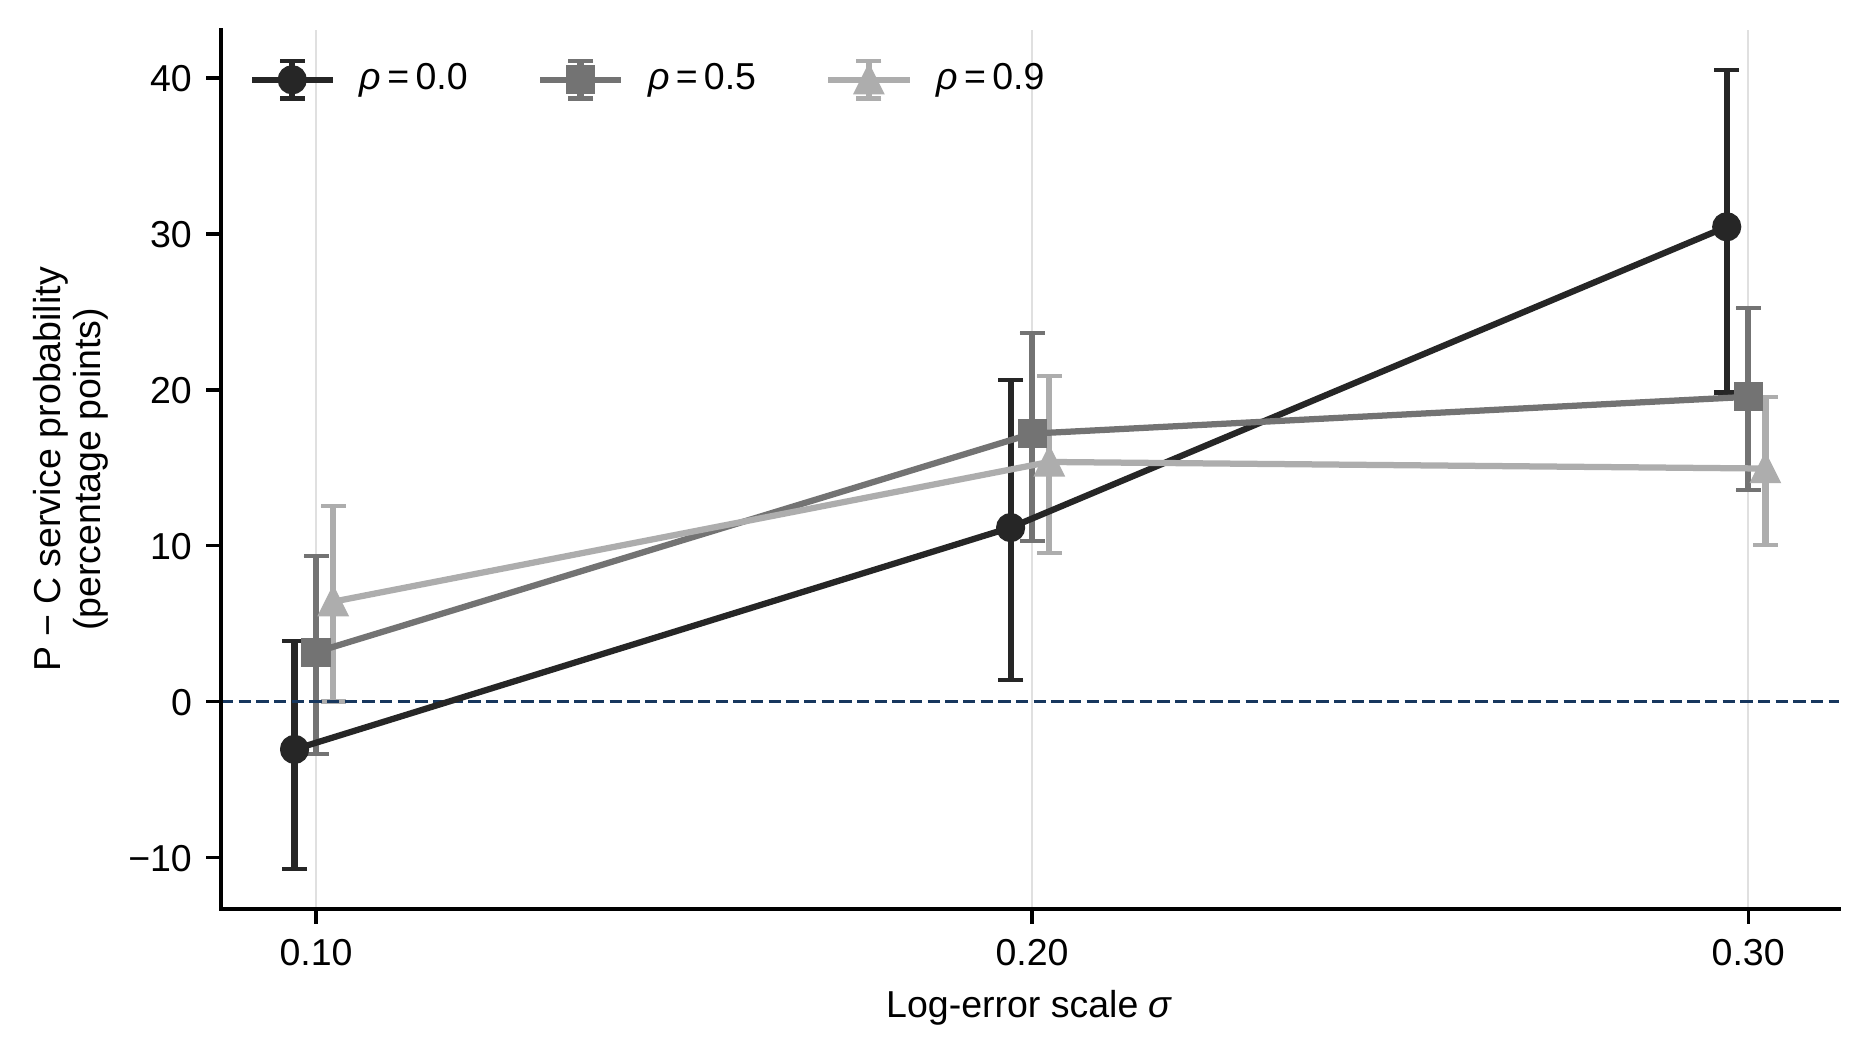
\includegraphics[width=0.85\textwidth]{Fig1.png}
 \caption{Difference in validated service probability between the original
 screening procedure (P) and 20\% padding (C) on the 46 development instances, as
 the random delay $\sigma$ and its correlation $\rho$ vary. Plans are fixed; error
 bars are 95\% bootstrap intervals over instances.}
 \label{fig:noise}
\end{figure}

\subsection{Padding at other levels}

A fixed 20\% pad may simply be the wrong amount, so Table~\ref{tab:padding} and
Fig.~\ref{fig:padding} repeat the comparison with padding from 0 to 50\%. Over all
instances, no padding level came close to the capped screening procedure. The best
level, 30\%, pooled 66.7\% against 86.6\%, a difference of
$-$19.9 points [$-$28.8, $-$11.7]. More padding did not keep
helping, because heavy padding makes many instances impossible to plan: the padded
planner found a plan on 34 of the 53 instances at 40\% and on only
26 at 50\%.

Where heavy padding did find a plan, that plan was reliable. On those 26
instances, 50\% padding served 96.1\% against 87.9\% for
screening, 8.2 points more [1.2, 16.1], and used
0.77 more vehicles per instance. These were the easier instances,
however, and on the other 27 the padded planner returned nothing. A
planner who fixes one padding level therefore has to choose between unreliable plans
at low levels and missing plans at high ones. Screening avoids that choice, because
it picks the buffer for each instance separately and the cap keeps every customer
reachable. At 30\% padding, where the padded planner did best overall, screening drove
3.1\% more distance than the padded plans on the instances where both
had a plan, so its extra reliability costs only a few percent of distance.

\begin{table}[t]
\centering
\small
\setlength{\tabcolsep}{4pt}
\caption{Padding every trip by a fixed percentage on the 53 development instances (exploratory). \emph{Plans}: instances on which the padded planner found a plan. \emph{All}: pooled service over all instances, an instance without a plan scoring zero. The next three columns use only the instances with a padded plan: the padded plans' service, the capped screening procedure's service on the same instances, and the difference (padding minus screening, percentage points, 95\% paired bootstrap interval). Distance (\%) and vehicles are also padding minus screening on those instances. Over all instances the capped procedure pooled 86.6\%.}
\label{tab:padding}
\begin{tabular}{@{}rrrrrlrr@{}}
\toprule
 & & \multicolumn{1}{c}{All} & \multicolumn{3}{c}{Instances with a padded plan} & & \\

Padding & Plans & Pooled & Padded & Screened & Difference & Distance & Vehicles\\
\midrule
0\% & 53/53 & 21.9 & 21.9 & 86.6 & $-$64.7 [$-$70.2, $-$58.8] & $-$7.1 & $-$0.89\\
10\% & 51/53 & 43.7 & 45.4 & 88.4 & $-$42.9 [$-$48.0, $-$37.4] & $-$6.2 & $-$0.59\\
20\% & 46/53 & 56.8 & 65.4 & 89.4 & $-$23.9 [$-$29.2, $-$18.2] & $-$4.8 & $-$0.22\\
30\% & 43/53 & 66.7 & 82.2 & 90.3 & $-$8.1 [$-$13.1, $-$2.4] & $-$3.1 & 0.21\\
40\% & 34/53 & 58.8 & 91.6 & 88.5 & 3.1 [$-$2.8, 10.0] & $-$1.0 & 0.47\\
50\% & 26/53 & 47.1 & 96.1 & 87.9 & 8.2 [1.2, 16.1] & 0.9 & 0.77\\
\bottomrule
\end{tabular}
\end{table}

\begin{figure}[t]
 \centering
 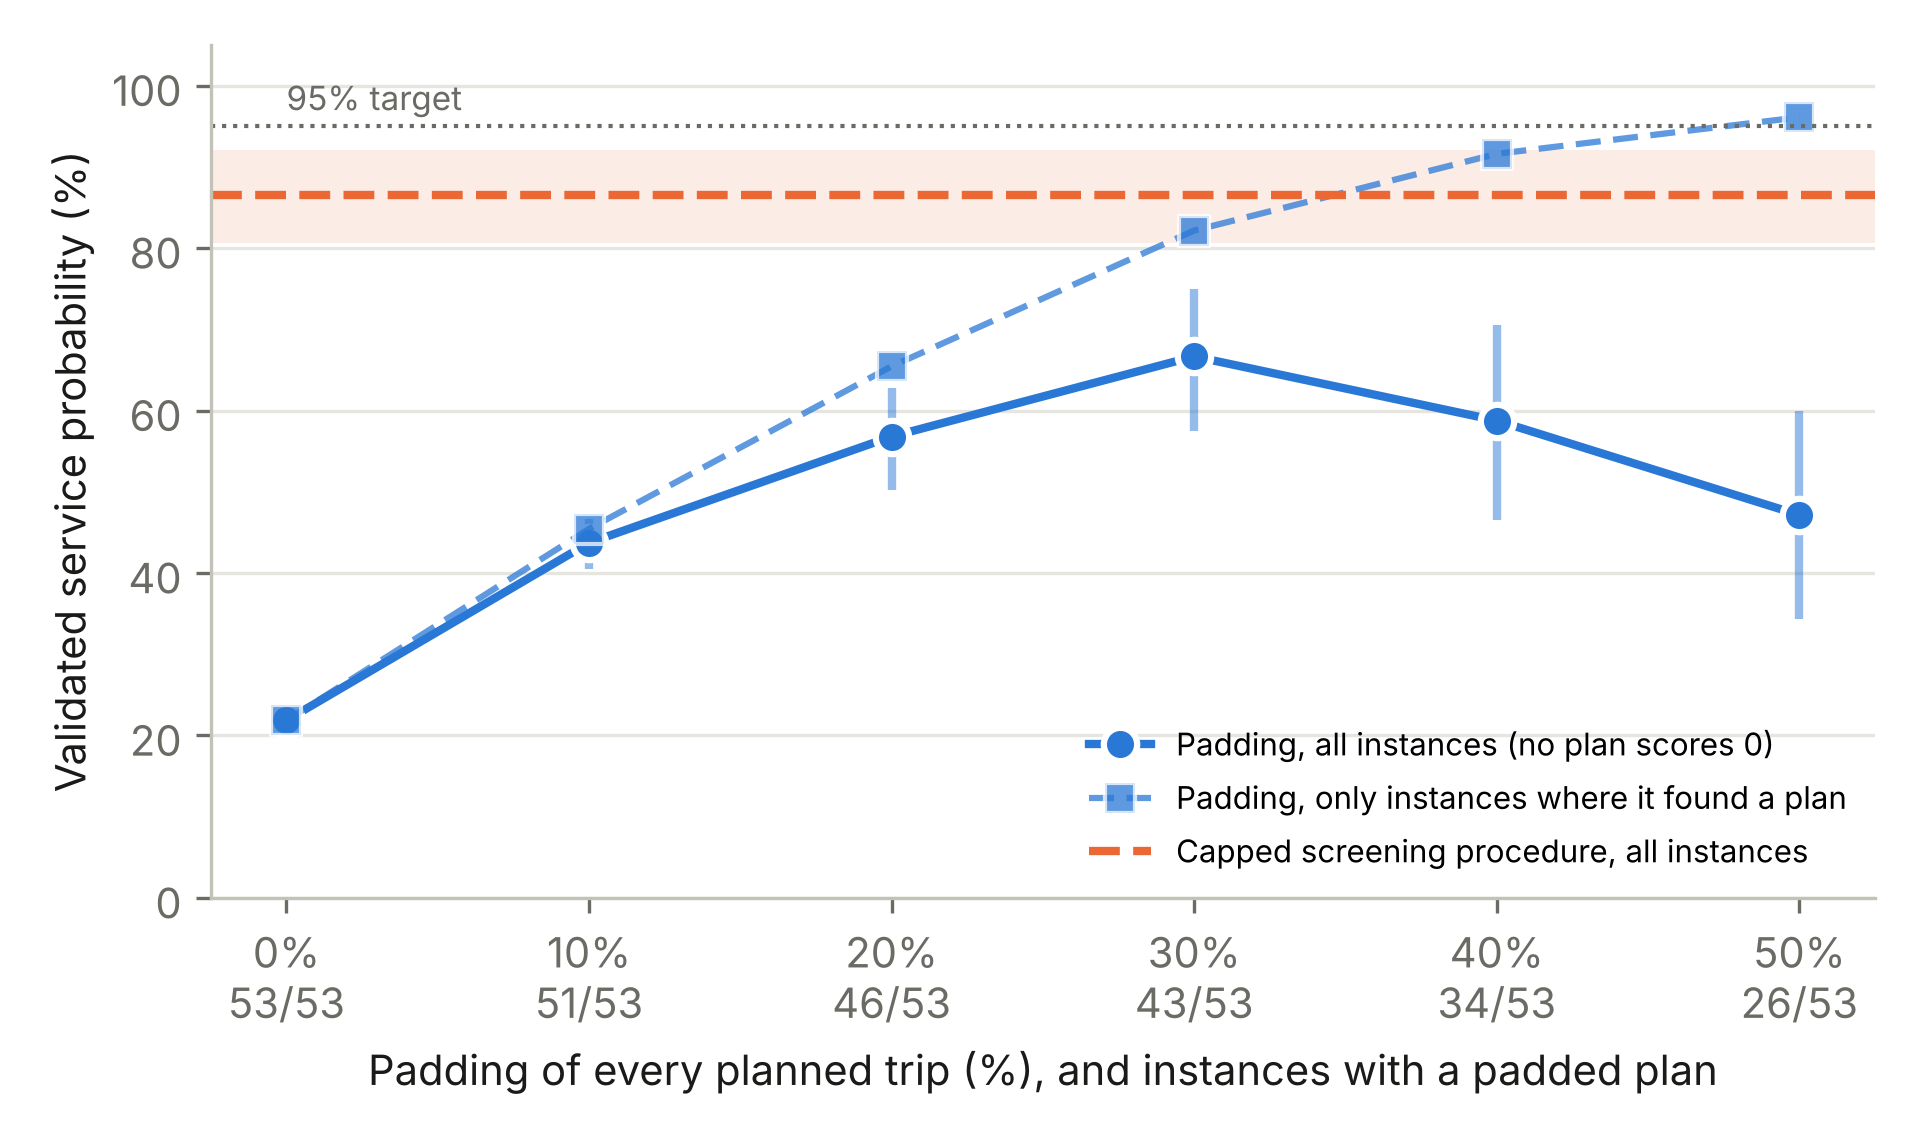
\includegraphics[width=0.85\textwidth]{FigPadding.png}
 \caption{Validated service probability against the padding applied to every
 trip, on the 53 development instances. The solid line counts an instance without
 a padded plan as zero; the dashed line uses only the instances where a padded plan
 exists (counts under the axis). The orange line and band show the capped screening
 procedure over all instances with its 95\% bootstrap interval.}
 \label{fig:padding}
\end{figure}

\subsection{The cap removes most failures}

On 21 development instances the original procedure found no plan that
passed the test, and on 17 of them the shortest-path test proved
that some customer had become unreachable at a large buffer. Capping
(Table~\ref{tab:screen}) raised the number of instances with a passing plan from
32 to 42, and pooled service by
7.7 [3.5, 12.5] points. At 100 and 200 customers the capped procedure found a
passing plan on every instance and pooled 97.5--97.6\%. It used
2.5\% more distance and 0.43 more vehicles on average
than the original procedure. Of the 42 plans that passed screening,
40 also kept a lower bound of at least 0.95 on the 5000 validation
days, which shows that the screen rarely admits a plan that later disappoints.

\begin{table}[t]
\centering
\footnotesize
\setlength{\tabcolsep}{4pt}
\caption{Development study, all 53 instances. For each procedure: instances admitted by screening out of all instances of that size, with the number whose lower bound also reached 0.95 on the validation bank in parentheses, and pooled validated service probability (\%) with a 95\% bootstrap interval, fallback plans included.}
\label{tab:screen}
\begin{tabular}{@{}rllllll@{}}
\toprule
 & \multicolumn{2}{l}{Original procedure} & \multicolumn{2}{l}{Screened conservative} & \multicolumn{2}{l}{Capped procedure}\\
$n$ & Admitted & Pooled & Admitted & Pooled & Admitted & Pooled\\
\midrule
20 & 14/20 (14) & 81.6 [70.2, 91.9] & 15/20 (15) & 87.7 [79.0, 94.7] & 14/20 (14) & 81.6 [70.3, 92.0]\\
50 & 8/15 (8) & 72.7 [59.2, 86.4] & 4/15 (4) & 67.5 [58.2, 77.3] & 10/15 (10) & 80.1 [66.9, 90.8]\\
100 & 6/10 (5) & 81.3 [68.8, 93.3] & 4/10 (4) & 77.5 [67.2, 88.2] & 10/10 (9) & 97.5 [96.7, 98.2]\\
200 & 4/8 (3) & 80.6 [68.7, 92.3] & 2/8 (2) & 78.3 [71.0, 86.5] & 8/8 (7) & 97.6 [96.9, 98.2]\\
\bottomrule
\end{tabular}
\end{table}

Pooled service stayed below the 95\% target because of the remaining instances,
all with 20 or 50 customers, where no candidate passed and a fallback was used.
Plans that passed averaged 97.4\% validated service, while the
11 fallback plans averaged 45.2\%.

\subsection{Confirmatory studies}

Table~\ref{tab:primaries} lists the eight primary hypotheses. Seven were confirmed.
In study~1, screening beat 20\% padding by 15.7 points on new instances,
and capping added 11.7 points. In study~2, with the stronger HGS solver,
capped screening beat padding by 28.0 points, so the gain does not depend
on a weak solver. The hypothesis that was not confirmed (G2) concerned a change to
the fallback: returning the padded plan when nothing passes did not measurably help
the capped OR-Tools procedure, because that procedure rarely needed a fallback.
Study~3 part B tested a different rule, returning the candidate that came closest to
passing, and it raised pooled service by 7.3 and 4.2 points for the two
solvers, to 94.4\% and 94.9\%.

\begin{table}[t]
\centering
\small
\caption{The eight primary hypotheses of the three confirmatory studies. Each was fixed and publicly timestamped before its instances were solved. Estimates are differences in validated service probability (percentage points) with 97.5\% paired bootstrap intervals over instances; a hypothesis is confirmed when its interval lies above zero.}
\label{tab:primaries}
\begin{tabular}{@{}cllll@{}}
\toprule
Study & & Contrast & Estimate [interval] & Decision\\
\midrule
1 & H1 & Original procedure minus 20\% padding (50 instances) & 15.7 [7.5, 23.6] & confirmed\\
1 & H2 & Capped minus original procedure (53 instances) & 11.7 [5.9, 17.9] & confirmed\\
2 & G1 & Capped procedure with HGS minus 20\% padding with HGS (49 instances) & 28.0 [23.0, 32.8] & confirmed\\
2 & G2 & Conservative minus slack-aware fallback, capped OR-Tools procedure & 0.4 [$-$0.7, 2.1] & not confirmed\\
3A & R1 & Screened robust model minus capped OR-Tools procedure (90 instances) & 6.7 [3.0, 11.1] & confirmed\\
3A & R2 & Screened robust model minus capped HGS procedure (45 instances) & 6.7 [2.2, 12.2] & confirmed\\
3B & F1 & Best-screened minus default fallback, capped OR-Tools procedure & 7.3 [2.3, 13.2] & confirmed\\
3B & F2 & Best-screened minus default fallback, capped HGS procedure & 4.2 [1.2, 8.0] & confirmed\\
\bottomrule
\end{tabular}
\end{table}

\subsection{Comparison with robust optimization}

A budgeted robust model plans against worst-case travel times on a limited number
of trips. Without a reachability correction it failed on 16 of
45 development instances at its most protective setting, for the same
reason the uncapped procedure failed. With the analogous correction and the same
screen, the robust plans were more reliable than both screened procedures in
study~3 part A (by 6.7 and 6.7 points; Table~\ref{tab:primaries}), but
they used 0.42 more vehicles per instance than the HGS procedure. When they
were limited to no more vehicles than the comparison plan, their advantage was no
longer statistically detectable. Screening is therefore not the most reliable
planner tested; its strength is that it works with any existing solver.

\section{Discussion}

The results support a practical point. A company that already uses a routing solver
can make its plans more reliable than a fixed 20\% padding without changing the
solver, by asking it for a few buffered variants and keeping the best one that
passes a simulation test. The test is cheap: screening a candidate took
3 to 24~ms, against several seconds to
generate it. Each accepted plan also comes with a stated, tested reliability, which
padding does not provide. The padding sweep shows why choosing the buffer per
instance matters: a fixed pad is either too small to protect most routes or so
large that many instances can no longer be planned. The reachability cap is a one-line change, and
Lemma~1 shows why it is safe; the same idea also rescued the robust
model.

The study has clear limits. The cities are synthetic squares and the delay model is
assumed, not estimated from real traffic data, so the percentages are not forecasts
for a real fleet. The confirmatory studies show that the findings repeat on new
instances from the same generator; they do not show that they hold in a different
city. The advantage also depends on the planner's objective: with equal weights on
the four quantities it fell to 6.3 points, with an interval that
included zero. The Wilson bound holds for each candidate separately, not for all 13
at once; a stricter Bonferroni version removed all 11 admitted plans that
later fell short, while 1 new selection fell short, at a cost of at most
2 admissions per study. Finally, vehicles always leave at their planned
times, and breakdowns and same-day replanning are not modelled.

Pooled service stayed just below 95\% because of the few instances with no passing
plan. Better candidates for those instances, for example from a solver that models
uncertainty directly, are the clearest next step, together with a test on real
travel-time data.

\section{Conclusion}

On simulated delivery problems with 20 to 200 customers, screening a family of
buffered plans from an ordinary solver gave more reliable service than padding every
trip by 20\%, with two different solvers; pooled over all instances it also beat
every fixed padding level from 0 to 50\%, and three confirmatory studies with
published hypotheses confirmed seven of their eight primary hypotheses. A simple cap
on the buffer, proved safe in Lemma~1, removed a failure that also
affects robust optimization. The method's main appeal is that it adds a measurable
reliability guarantee to the tools companies already use.

\section*{Acknowledgments}
The author thanks the researchers who answered methodological questions by e-mail
during the project. Generative AI assistants (OpenAI's ChatGPT and Anthropic's
Claude) were used for code development, code review, checking the analysis, and
drafting and editing text; every experiment was run from the archived code, every
number regenerates from the archived records, and the author takes full
responsibility for the content. All code, instances, records and analysis scripts
are openly available\cite{ali2026archive}.



\end{document}
